\documentclass{proc} %Try article here.
\usepackage[margin=1in]{geometry}
\usepackage{graphicx}

\title{Graphics in \LaTeX}
\author{Abhishek Raj}
\date{\today}

\begin{document}
	\maketitle
	
	\section{Introduction}
	Picture books are just \emph{better}.
	
	\subsection{Including Graphics}
	This is a banana in a JPG.
	
	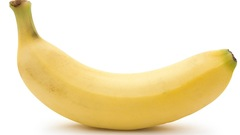
\includegraphics[width=2in]{Banana.jpg}
	
	This is a fish, in a PNG.
	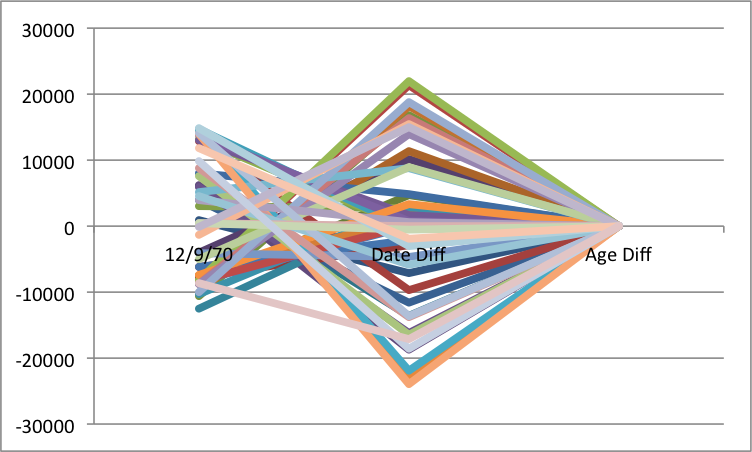
\includegraphics[width=2in]{Fish.png}
	
	\subsection{Float:Figure environment}
	In my article, I want to include a JPG image of a banana. You can see this image in the figure \ref{fig:banana}.
	
	\begin{figure}[htbp]
		\begin{center}
			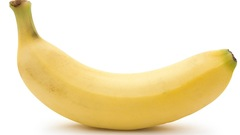
\includegraphics[width=2in]{Banana.jpg}
		\end{center}
		\caption{This is a banana.}
		\label{fig:banana}
	\end{figure}
	
	In my article, I want to include a png image of a fish. You can see this image in the figure \ref{fig:Fish}
	
	\begin{figure}[htbp]
		\begin{center}
			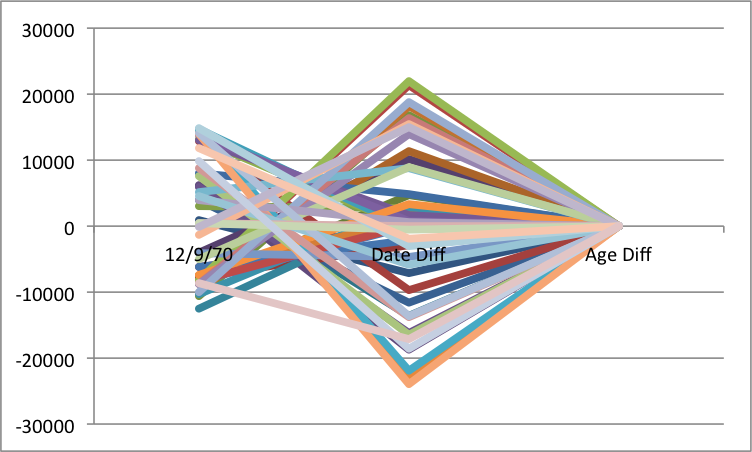
\includegraphics[width=2in]{Fish.png}
		\end{center}
		\caption{This is a Fish.}
		\label{fig:Fish}
	\end{figure}
	
	\section{Conclusion}
\end{document}
